\documentclass[frames,ps,pdf,slideColor,colorBG,accumulate]{prosper}
\usepackage[francais]{babel}
\usepackage{amsmath, amsfonts, amsbsy, pstricks, pst-node, pst-text, pst-3d}
\usepackage{graphicx,color,caption2,amssymb,pstricks,lmodern}
\usepackage{moreverb,epsfig,color,subfigure}
\NoFrenchBabelItemize
\usepackage{ucs}
\usepackage[utf8x]{inputenc}

\usepackage{pst-plot}
\usepackage[metapost]{mfpic}
\opengraphsfile{figs}



%\usepackage{epsfig}

%\documentclass[pdf,autumn,slideColor,colorBG]{prosper}
\title{Initiation à la recherche}
\subtitle{Soutenance}

\author{A.\textsc{Marguerite} R.\textsc{Rincé}}
%\Logo{
\includegraphics[scale=0.40]{img/logouniv.eps}}
\Logo(9,-0.7){
\includegraphics[scale=0.5]{img/logouniv.eps}}


\institution{
  Université de Nantes \\
  2 rue de la Houssinière, \\
  BP92208, F-44322 Nantes cedex 03, FRANCE
  
}

% Optional: text to put in the bottom of each slide.
% By default, the title of the talk will be placed there.
%\slideCaption{\textit{Rouben Rostamian, UMBC}}






%\NoFrenchBabelItemize
\begin{document}

% make the title slide
\maketitle



\overlays{7}{
  \begin{slide}{Presentation du laboratoire \textsc{LINA}}
    {Goal}: easily make presentation-quality slides \\
\begin{center}
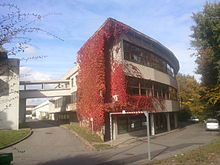
\includegraphics{img/lab.jpg}
\end{center} 

    \FromSlide{2}{\yellow Options}: \FromSlide{3}
    \begin{Itemize}
    \item PowerPoint \FromSlide{4}- what to do about equations?
      \FromSlide{5}
    \item \LaTeX $\rightarrow$ pdf  -several packages will do this
      \begin{Itemize}
        \FromSlide{6}
      \item pdfslide or P$^4$ with pdflatex
        \FromSlide{7}
      \item \texttt{prosper} - most straight-forward; can easily convert existing \texttt{seminar} slides
      \end{Itemize}
    \end{Itemize}
  \end{slide}
}



%% \begin{slide}{Présentation du laboratoire LINA}
%% \begin{minipage}{4cm}
%% dsqd
%% \end{minpage}
%% \begin{minipage}{7cm}
%% \begin{Itemize}
%% \item Item 1
%% \item Item 2
%% \item Item 3
%% \end{Itemize}
%% \end{minipage}
%% \end{slide}

%}  % closing brace of \overlays


\end{document}
